%(BEGIN_QUESTION)
% Copyright 2011, Tony R. Kuphaldt, released under the Creative Commons Attribution License (v 1.0)
% This means you may do almost anything with this work of mine, so long as you give me proper credit

A {\tt NAND} logic function may be built up from a regular {\tt AND} function plus an inverter function (a {\tt NOT} gate) on the output:

$$\includegraphics[width=15.5cm]{i04092x01.eps}$$

The same strategy of ``building'' a {\tt NAND} gate may be done in PLC ladder-diagram programming, by combining a normally-closed contact instruction with two contacts in series.

\vskip 10pt

Examine these two Allen-Bradley PLC programs, and explain why the left-hand program is ``wasteful'' while the right-hand program makes more efficient use of available bits:

$$\includegraphics[width=15.5cm]{i04092x02.eps}$$

Examine these two Siemens S7 PLC programs, and explain why the left-hand program is ``wasteful'' while the right-hand program makes more efficient use of available bits in the same ways the Allen-Bradley example programs were wasteful/efficient:

$$\includegraphics[width=15.5cm]{i04092x03.eps}$$

\vskip 10pt

\noindent
{\bf Note: many novice PLC programmers commit this error of ``wasting'' valuable I/O as they write their programs!}


\underbar{file i04092}
%(END_QUESTION)




%(BEGIN_ANSWER)

Each ``wasteful'' program uses an output bit as the intermediary bit between the {\tt AND} and {\tt NOT} functions when there is no need.  

%(END_ANSWER)





%(BEGIN_NOTES)

Output I/O points are valuable because they (and they alone) can be used to drive real-world devices on and off.  No need to ``waste'' them on functions that have no real-world application, when we may use bits that are internal to the PLC's memory!

%INDEX% PLC, ladder logic program analysis and explanation (Allen-Bradley)
%INDEX% PLC, ladder logic program analysis and explanation (Siemens S7)

%(END_NOTES)


